\documentclass[12pt, a4paper]{report}
%\usepackage[communication, french]{idiap}	
\usepackage{graphicx}
\usepackage{psfrag}
\usepackage{epsfig}
\usepackage[hang,small,bf]{caption} 
\usepackage{amsmath,amssymb}

\setlength{\captionmargin}{50pt}

% MARGES
\setlength{\hoffset}{-0.4in} \addtolength{\textwidth}{1.1in}
\setlength{\voffset}{-0.4in} \addtolength{\textheight}{0.2in}

\begin{document}

\begin{center}
\thispagestyle{empty}

\begin{figure}[h]
\centering
\begin{minipage}{5cm}

\includegraphics[width=1\textwidth]{logo-fundp.jpg}
\end{minipage}
\hfill
\begin{minipage}{5cm}

\includegraphics[width=1\textwidth]{Idiap-logo-E.png}
\end{minipage}
\end{figure}

\centering
\vfill

\Huge{\textbf{Automatic true-false question answering in meetings}}\\
\vspace{7mm}
\Large{\textsc{Le Quoc Anh}}\\

\vspace{3mm}
%Master of Science Thesis\\
Master Internship Plan and Summary \\
\normalsize
\vspace{3mm}
University of Namur \\
Faculty of Computer Science \\
\large

\vfill
\begin{tabular}{l l l}
Supervisor: & Dr. Andrei Popescu-Belis &  (Idiap Research Institute)\\
& & \\
Professor : & Prof. Jean-Paul Leclercq & (University of Namur, FUNDP)\\
\end{tabular}

\vfill
\normalsize
1 August 2008 -  31 January 2009
\end{center}

%\title{\vspace{-5cm}
%        \LARGE{Master Internship Plan and Summary\\}
%        \vspace{6cm}
%        \LARGE{\emph{\texttt{Project title:} \textbf{Automatic true-false question answering in meetings}}}\\
%        \vspace{5cm}
%}

%\author{\vspace{3cm}
%\begin{tabular}{ll}    
%    \small \texttt{Supervisor 1:}      & \small Dr. Andrei Popescu-Belis (Idiap)\\
%    \small \texttt{Supervisor 2:}			 & \small Prof. Jean-Paul Leclercq (FUNDP)\\		%			
%    \small \texttt{Trainee:}          & \small Quoc Anh LE \\
%    \small \texttt{Duration:}& \small Six months (1 August 2008 -  31 January 2009)\\    
%    \small \texttt{Email:}           & \small quoc-anh.le@idiap.ch - lequocanh@fundp.ac.be\\
%\end{tabular}}



\newpage
\tableofcontents

\newpage
\listoffigures



\chapter{Introduction}

Internship is considered as the third semester of master programme of Computer Science at the University of Namur (FUNDP). In the frame of this activity, I chose Idiap as an ideal place for my internship, which will be introduced in detail in the following chapter (chapter 2). My internship at Idiap lasts for 6 months, from 1 August 2008 to 31 January 2009, under the supervision of Dr. Andrei Popescu-Belis, senior researcher at the Idiap Research Institute and Prof. Jean-Paul Leclercq at the Faculty of Computer Science, University of Namur.\\

The objective of my internship subject entiltled "Automatic true-false question answering in meetings", is to build a system which can identify the true statement in a pair of two analogous true-false statements concerning the information of a meeting transcript. The project consists of two phases: the first is to locate the region of transcript that is the most likely to contain the answer and in the second phase, the retrieved region from the first phase will be analyzed in order to give the answer. These two phases will be shorly described in chapter 3. In addition, a plan of future work will be proposed as well.\\

After three months working here, some results are obtained for the first phase. These results will be presented in the chapter 4. \\

The last chapter is a conclusion.

\newpage
\chapter{Presentation of Idiap} 
 
The Idiap Research Institute \cite{6}, initially referred to as "Dalle Molle Institute for Perceptual Artificial Intelligence" (Institut Dalle Molle d'Intelligence Artificielle Perceptive) was founded in 1991 by the Dalle Molle Foundation. In November 1996, Idiap officially became a Research Foundation, with the following co-founders: the City of Martigny, the State of Valais, the Swiss Federal Institute of Technology at Lausanne (EPFL), the University of Geneva and Swisscom.

Active in the areas of multimodal interaction and multimedia information management, the institute is now the leader of the Swiss National Center of Competence in Research IM2. Idiap's activities follow a triple objective: (i) conducting fundamental research at the highest level in its areas of expertise, thus ensuring a leading role nation-, european-, and world-wide; (ii) providing education for young researchers through the hiring of PhD students but also by attracting talented undergraduates to discover the world of research; (iii) transfer of knowledge and technologies to guarantee the best possible dissemination of research results in the scientific world and within strong collaboration with industry.

At this moment, there are 95 people (including about sixty researchers) from 23 nationalities working regularly at the Idiap. The success of the Idiap is shown by more than one hundred scientific publications in journals and conferences annually and approximately 80 new technical reports every year, available on the Idiap web site.

\newpage
\chapter{State of the art}

\newpage

\chapter{Presentation of project} 
\section{Overview}
Archives of meeting recordings are useful to check or to retrieve information from past
meetings. However, such archives are usable only if appropriate tools, generally named
meeting browsers, are available to locate the information that is searched for. One
approach to meeting browsing is to design general-purpose browsers that help human
users to locate relevant information. In addition, another possibility is to design browsers that
locate information automatically, for instance for verification (fact checking) purposes.\\

The goal of this internship project is to design such an automatic browser, and to assess
its performance on a set of pairs of true-false statements, which have been initially used
to evaluate human-directed browsers.\\

In other words, the goal is to design and to implement a system that determines the true
and the false statement in each pair, to evaluate its performance over a set of several
hundreds such pairs (for 2 recorded meetings), and to compare it with human subjects
using existing meeting browsers. A comparative analysis of the system and the human
scores on specific questions should indicate whether or not system and humans have the
same difficulties answering such questions. This work will thus provide a baseline score
against which humandirected browsers must be compared, to demonstrate significant
improvement over a fully automated tool.\\

\subsection{Meeting transcript}
Two meeting transcripts are used to test the system (IB4010 and IS1008c). They are selected from the AMI Corpus (\emph{http://mmm.idiap.ch}) for the observation collection procedure. The meetings are dicussed in English and involve four participants, native or non-native English speakers. In the first meeting IB4010, managers of a movie club discuss to select the next movie to show; meanwhile, in the second one IS1008c, a team discusses the design of a remote control. \cite{4}

The transcripts was made by hand in detail, indicating correctly the time speaking, as well the speakers for each conversation in the meeting.

Example:
\small
\begin{verbatim}  

[0:49][0:56] denis : So I don't know if you all received the the a- agenda for this meeting. 
[0:49][0:56] denis : Do you - no? 
[0:55][0:56] mirek : No, I haven't. 
[0:57][0:57] denis : Here it is. 
[0:57][0:57] mirek : Thank you.
[0:58][0:59] agnes : I haven't
[0:59][1:27] denis : So the goal for today are
\end{verbatim}
\normalsize

\subsection{Observations}
They are a set of pair of two analogous true-false statements concerning the information of a meeting transcript. They are also called \textit{observations of interest}. These questions, used in testing, are produced by a set of observers, who independently watch selected meeting from corpus. The observers have available full recordings from every media source, in parallel, including paper printouts of the slides accompanying the meeting. \cite{3}

Each observation is stated as a complementary pair of statements, one true and one false. In fact, at the first time, observer creates list observations and then he creates a false version of each. Observers are instructed to produce observations that should not be easy to guess without using the meeting information. Then the observations should be simply and concisely stated.

Each observation is time-stamped with the media time into the recording, and summitted with an estimate of its locality: \textit{here, around, throughout} \cite{5} in which one observation is marked \textit{here} by observer if it is pertinent to that particular moment, \textit{around} if it covers at least a minute of the meeting around the point the observer have selected and \textit{throughout} if it broadly covers the whole meeting. However, in this system, the questions whose type is \textit{throughout} are avoided because it is difficult to determine the answer by using lexcial similarity algorithm - this algorithm is described in the next chapter. Besides, the algorithm only tested with the questions which were accepted by examinants (\textit{reject = A}).

The database is stored at the server of Idiap (\emph{http://pneumatix.idiap.ch/phpmyadmin}). The questions are extracted from the table \emph{observations} in the database \emph{bet} by the SQL command:

\small
\begin{verbatim}  
SELECT scope, trueStatement, falseStatement 
FROM observations 
WHERE	reject = 'A' AND 
	meeting = 'IB4010' AND 
	scope !=  'Throughout' 
ORDER BY 'mediaTime'


1
Here
Denis was interested in whether participants have received an agenda for the meeting
Agnes was interested in whether participants have received an agenda for the meeting
---------------------------
2
Around
Mirek had not received the agenda for the meeting
Andrei had not received the agenda for the meeting
\end{verbatim}
\normalsize

In the trial run, the system uses about 200 observations (pairs) from six observers of two about 40-minute meetings. In order to improve the speed of performance, the extracted database is stored in the local computer. Later, the question filed will be modified to add information of correct answer made by hand corresponding to each pair of questions. 



\section{Plan of work}


The project proceeds in two phases. The first phase identifies the section of the meeting transcript which is most likely to contain the answer (i.e. the facts that discriminate between the true and the false statement), using lexical similarity of pre-processed transcript windows and statements. The second phase compares the two candidate statements with respect to the identified paragraph(s), and hypothesizes the true one. The project integrates some open sources in order to analyse the lexical system. They will be described in detail in the following sections.\\

 The result of Internship Project is supposed to be developped in my Master thesis and defended in June, 2009 at the Faculty of Computer Science, University of Namur. 
\subsection{Phase 1 - Passage Retrieval}

The objective of this phase is to design an accepted algorithm to retrieve the best snippet in the meeting transcript in order to be able to assess the true-false state for each statement.

This first phase is planned to last 3 months (1 August 2008 - 1 November 2008). Some results of this phase to be obtained so far is reported at the chapter 4. 


\subsubsection{Proposed algorithm}
Generally, the questions answering systems use the lexical similary as an accepted solution. However, each problem in particular applies this method in different ways in order to accord with features of their problem.

Before doing the algorithm, the transcript and the questions are pre-processed in order to reduce the number of calculations: removing stop-words and characters not related to words - punctuation signs such as comma, dot, quotation mark, semicolon or exclamation (':' , ',' , '!' , '\^',...) and in order to standardize the text (converting abbreviated words into full forms: \textbf{I've} becomes \textbf{I have},... and converting numeric form to text: \textbf{2nd} becomes \textbf{second}, \textbf{12} becomes \textbf{twelve},...). Then, both the question and the transcript are transformed into sequences of terms (words), which are to be matched one into another. Finally, stemming normalizes different morphological forms of words into a common feature. A question term matches a transcrip term if they have the same stem.

The stop-words list was taken from the site \emph{(http://www.ranks.nl/resources/stopwords.html)}, that is based on what they believe to be Google stop-words. Those are words which are ussually ignored if we search for them in combination with another word. This list was modified a bit like this: \emph{a, about, an, are, as, at, am, and, be, by, for, how, in, is, it, of, on, or, that, the, they, this, to, so, uh, um, really, very, was, were, we, well, will, with, wow}.

In this project, an indexed-inverse words method was proposed that pays attention to use some features of a meeting. Those are speaker and synonyms for each indexed word. The words are indexed with their position in the transcript before removing the stop-words such as a table of contents a book. So, firstly, the algorithm works with the indexes, after that, it retrieves the real position of found words in order to compare those with the reference answer who was found in the transcript by hand that for the objective of answer evaluation. An example for transcript table can be described as follows:

\begin{figure}[htbp]
\centering
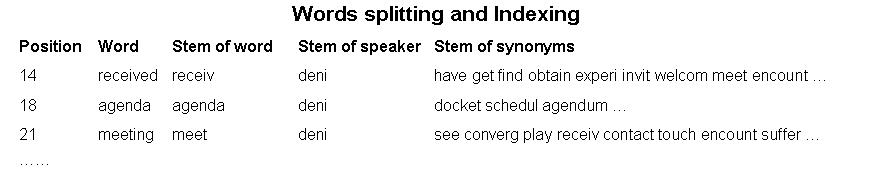
\includegraphics[scale = 0.7]{index.jpg}
\caption{Words splitting and indexing}\label{fig1}
\end{figure}

All database is stored in the dynamic memory (RAM) in order to speed execution when the algorithm is experienced with variable parameters.

One important remark of meeting transcript, which is different from texts using in the other questions answering systems is that the presence of participants, so the definition of which sentence belongs to which participant are very important to answer the question. That is why, when we calculate the score of word matching between one search window and one question, the score of name matching is 2.0 while the score of others is 1.0. Moreover, the synonyms is considered less important so its score is 0.2. 

For the size and step of search window size, its unit of calculation may be sentence or word. There are two methods to set the parameters for search window size and search window step: dynamic method depends on the size of the question and the size of transcript and static method  is contrary to the dynamic method. For example:  Search window size = 5* number of words of the question or  search window step = number of words of the question.

%The way they speak in meeting is spoken language, so the grammar is not formal in most of conversations and even not correct. Sometimes the participants repeat some words many time in one sentence. Because of that, frequence of one found word was not used as one factor incressing the total score when the algorithm calculates the score of one search window but counting the common words between the question and searh window. However, if one word repeats more than one time in both the search window and the question, the score must be calculated by the number of time they appear in the both two texts. 

The above algorithm which calculates the score of each search window can be described in pseudocode as follows:
\small
\begin{verbatim}
	for each word_question in the question
	for each index in the window of transcript table
		if (word_question == speaker)         {score = score + 2.0; break;}
		if (word_question == stem)             {score = score + 1.0; break;}	
		if (word_question belongs to synonyms) {score = score + 0.2; break;}
\end{verbatim}
\normalsize		
		
\textit{Remarks}:
\begin{enumerate}
\item {The priority order is given to “speaker matching”, then “stem matching” and 
   lastly “synonyms matching” in order to bring the highest score for the search window.}
\item {The frequency of one found word is not used to increase the score but in the 
   case “multiple matching”, if one word repeats more than one time in both the 
   question and the transcript, the score will be calculated as the minimum number 
   of appearance of this word between the question and the transcript.}
\end{enumerate}


The following schema presents the processing flow of the first phase. 

\begin{figure}[htbp]
\centering
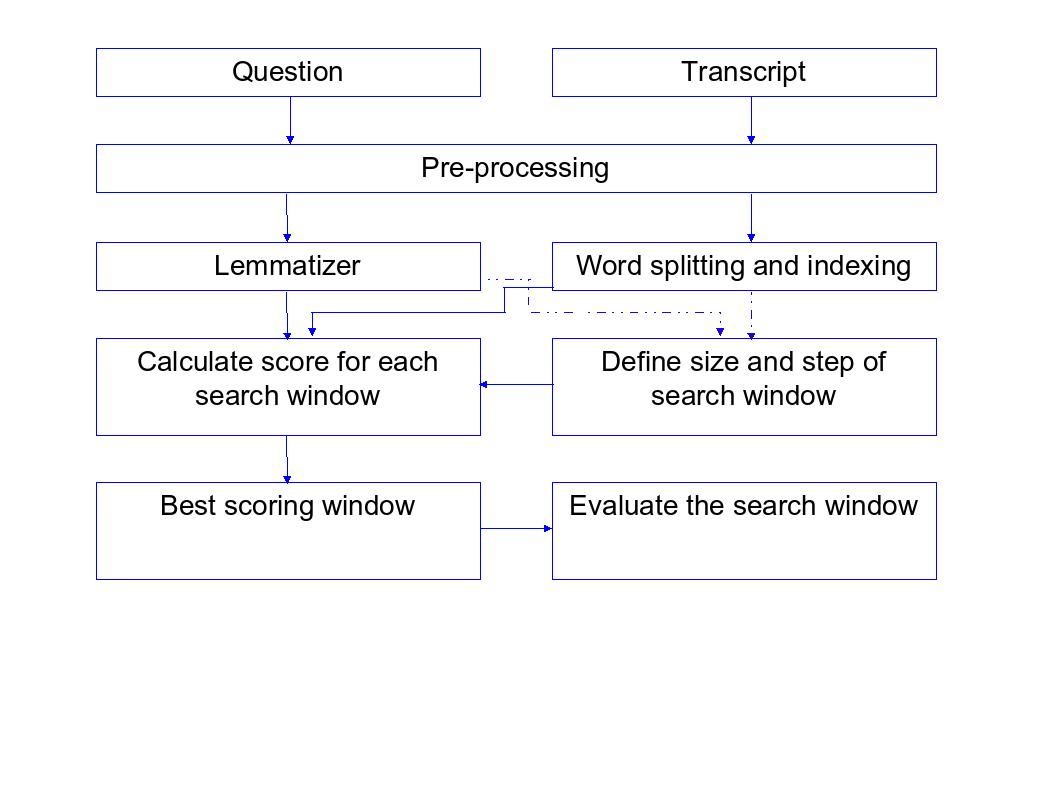
\includegraphics[scale = 0.4]{schema1.jpg}
\caption{The first phase - Passage Retrieval}\label{fig1}
\end{figure}
\newpage



\subsection{Phase 2 - Passage Analysis}
The objective of the second phase is to analyse the retrieved passasges from the first phase in order to assess the true statement in the pair.

The planned period of this phase is 2 months (1 November 2008 - 1 January 2009). The last month of internship will be used to experience the system and to write reports.

We have two cases in the results of the first phase: correct passage, which can help us to assess the true statement and false passage that can not certainly help us to find the answer. However, we can not know whether a retrieved passage is correct or not. So the proposed algorithm is supposed that the retrieved passage always contains the significationt that helps to discriminate the true statement. In the case of fault from result of phase 1 - passage retrieval algorithm, result of the phase 2 is random. Two retrieved passasges correspondent to two questions in one pair may be the same passage or two different passage, but it is not important. The proposed algorithm uses score of retrieved passage in order to assess status of correspondent statement. The question whose higher score of the passage will be considered true. In the case of the same score of two passage, the passage retrieval algorithm will be repeated in which two consecutive words are used as the unit matching indeed of one word. After that, if the two retrieved passages still have the same score, we have to analyse the questions from its context but this is a difficult problem concerning Nature Language Processing (NLP). The following schema presents the proposed algorithm.

\begin{figure}[htbp]
\centering
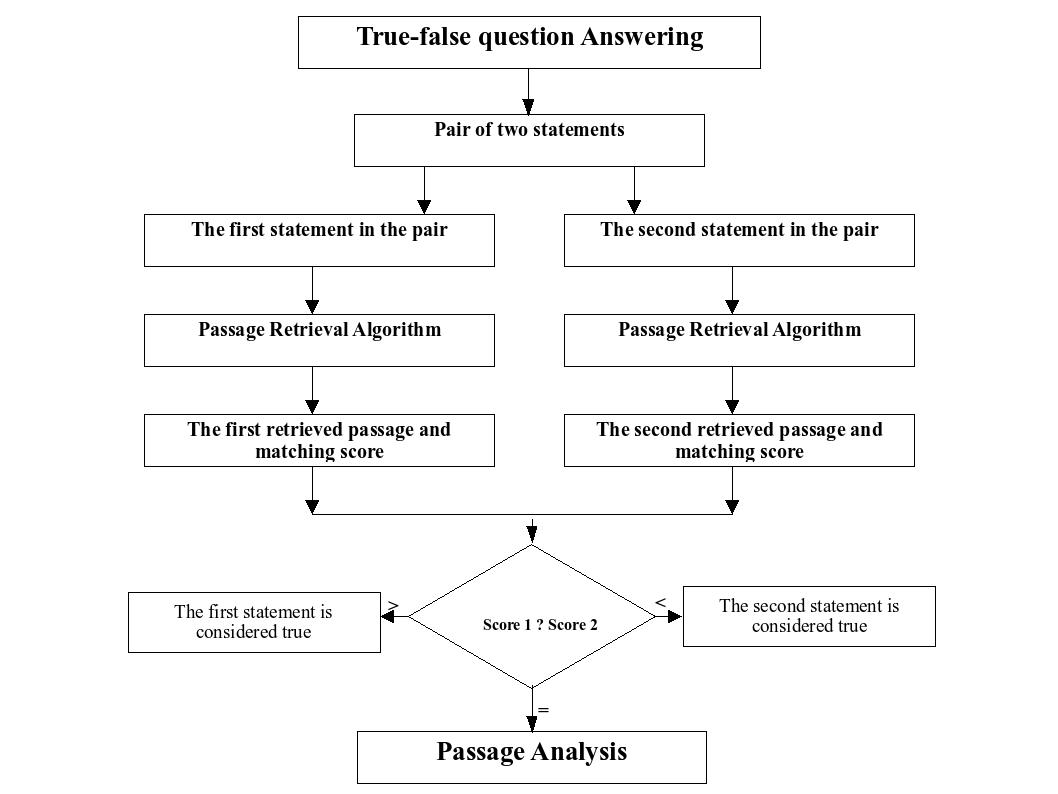
\includegraphics[height=9.5 cm]{schema2.jpg}
\caption{The second phase - Passage analysis}\label{fig5}
\end{figure}
\newpage


% The classical measures are \textit{precision} and \textit{recall} (van Rijsbergen, 1979). Recall is the fraction of the relevant documents from the collection that are retrieved, thus testing the system's ability to retrieve all relevant documents. Conversely, precision is the fraction of the retrieved documents that are relevant, thus testing the system's ability to retrieve only relevant documents. Precision and recall are real-valued variables in the interval [0,1]. An ideal system has 1-values for precision and recall, in other words it returns all of the relevant documents, and only the relevant documents.

% term is different from word: ex: `how much' is a term but it is not a word, it consists of two words

% a lexical term consists of the original word used in the question (e.g. knew), its part of speech - lemma (e.g. VBN standing for verb in past participle), the position of the word in the question and the word's morphological root - stem (e.g., know for the known). => original | type of word (verb, noun, adv, adj,..) | pos | lemma

% Lexical terms are classified into content and non-content terms. Content terms include nouns, verbs, adjectives and adverbs, and form the foundation for the higher-lever representation layers. Non-content words are auxiliary verbs (e.g., am or has), modal verbs (e.g., could, must), prepositions (e.g., for), conjunctions (e.g., and), interjections or pronouns (e.g., you). These ``small'' words have less importance in answer extraction but are nevertheless useful for other information processing tasks and also for question anwering as shown in later chapter.

\subsection{Tools}
\subsubsection{WordNet}
WordNet has an important informative role whenever the question keywords alone can not determine an acceptable answer. In this case, WordNet provides means for generating keyword alternations. Wordnet enables three forms of keyword alternations, as shown below \cite{2}:

\begin{enumerate}
 \item {Morphological alternations, to match different forms of the same irregular verb (lemmatizer). For example:   Three words 'had', 'has' and 'have' are the morphological alternations of the verb 'have'.  }
 \item {Lexical alternations, to match various forms of the same synset (synonym words). For example: The words 'movie', 'film', 'picture', 'pic', 'flick' are synonyms of the word 'movie'. }
 \item {Semantic alternations, to match words that are semantically related in the context defined by the question and the text passage (hyponym words,...)}
\begin{figure}[htbp]
\centering
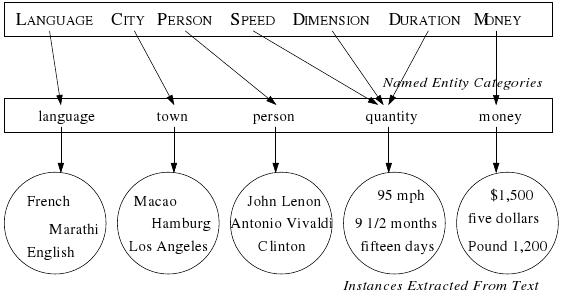
\includegraphics[height=6 cm]{wordnet_hyponyms.jpg}
\caption{Example of hyponym words in WordNet}\label{fig0}
\end{figure}
\end{enumerate}

\subsubsection{Snowball}
Snowball is a useful tool for word stem, which is a part of a word and common to all its inflected variants. That is why we can use it for word matching whenever two words are compared.
Examples \circle{7}:
The stem of the verb \textbf{wait} is \textbf{wait}: it is the part that is common to all its inflected variants: \textbf{wait} (infinitive), \textbf{wait} (imperative), \textbf{wait} (present, 3rd, singular), \textbf{wait} (present, other person and/or plural), \textbf{wait} (simple past), \textbf{wait} (past participle), \textbf{wait} (progressive).


\newpage
\chapter{Parameter optimization}
A technique of machine learning using training data and test data is applied in order to calculate the best parameters of search window (size and step).
The questions are splitted up into training data set and test data set in which we use 80\% of questions for training data and the remains for test data. The training data is taken in the way random from question set by dividing the question set into five parts and taking 4 parts.
In the first time, the programme search for the best parameters of search window by looping the algorithm on the traning data set with variable parameters (from 1xL to 20xL for window size and from 1 to L for window step). After that, these parameters will be applied to the test data set in order to evaluate leur performance.
The procedure is looped five times for variable test data corresponding to five parts of question set. Finally, performance obtained for each pair of parameters is calculated on the average of 5 results.
Peseudo code:

\newpage
\chapter{Definition of difficult level of questions}
One step qui takes a lot of time is the definition of difficult level of questions. The objective is to evaluate the performance of algorithm and also to help understand and improve the algorithm.

1. Source d'erreur

2. Definition of facile or difficile 

Qu'est-ce que ca montre?

Ca montre la limite de l'algorithme en utilisant lexical similarity

\newpage
\chapter{Word frequence}
Why they use log for tf-idf?
tf(i,j) = term(i) frequency in the given document(j) / length of document(j) (number of occurrences of all terms in document)
idf(i) = log(total number of document in the corpus / number of documents where the term(i) appears)

Then tfidf(i,j) = tf(i,j) x idf(i), so we can see that the higher term frequency (in the given document), the higher tf-idf, and the less document frequeny of the term in the whole collection of documents; the higher tf-idf.

However, in meeting transcript, there are some different features:
- spoken language:
- one short unified document, that means it tells about one topic particularly and there are relations between paragraphs.
That's why 

\newpage
\chapter{Experimental results}
\section{Phase 1 - Passage retrieval}
Definition of a passage: A passage can simply be defined as a sequence of words regardless sentences or paragraphs. 
The passage should be in a fixed range of sizes based on number of words, not too long or too short. Here, we define a passage, or a window, as a fixed-length sequence of words.
We can als consider sentences instead of words as the basic unit, and use heuristics to bound their lengths. Someone define a passage as a block of 30 words.
The main advantage of window-based passages is that they are easy to construct, irrespective of the text. However, there are disadvantages. If window-based passage are retrieved and presented to the phase 2, the context is sometime not clear to assess the question.

We work here on passage detection: 
- Passage detection attempts to identify passage related to user specified topics (category), while passage retrieval concerns with passages related to user queries.
- In passage detection, training documents are used to train a classifier on a topic, while passage retrieval is generally not a supervised process.
- In passage detection, the effectiveness of results depends on the accuracy of the text classification model. In passage retrieval, the effectiveness of results depends not only on the engine but also on how the query is formulated by a user.

Because of particularities of this problem, we work on passage detection instead of passage retrieval (passage retrieval tends to retrieve all passages containing the answer).
	- the user query is under form of a statement (true or false)
	- there is only one passage correspondent to a question (it doesn't exists more one correct passage for one question)
There are 3 document splitting approaches namely \textit{non-overlapping window} passage approach, \textit{overlapping window} approach and \textit{discourse passage} approach and mapped them to the problem of passage detection.
The \textit{non-overlapping window} based passage approach defines a passage as \textit{n} number of words (the first passage starts from 1 to n, and the second starts from n+1,...). In \textit{overlapping window} passage approach, a document is divided into passage of evenly sized blocks by overlapping n/2 words from the prior range and n/2 words from the next range. \textit{Discourse passages} are based on logical components such as discourse boundaries such as a sentence.
The best method for document splitting in detectiont task called \textit{dynamic windowing}. In earlier methods, we did not use the information regarding the meaning of query. So this feature will be applied to detect potential passages. For a fixed length of the passage that is n words long, we define a passage from n/2-1 terms before a transcript term found in the question and up to n/2 terms after that term. Hence, we make sure that each passage has at least one common term with the question.
\subsection{Fingure}
This demonstration describes effect of linguistic modules on system performance. 
Using the same parameters of window size and window step (those parameters are extracted by optimizing with machine learning technique described above).
\textbf{Baseline score} The baseline score describes the score that a system would achieve without any extension or analyse of word semantics. 
\textbf{Using stem}
\textbf{Using stem + synonyms}
\textbf{Using stem + synonyms + speaker factor}
\textbf{Using stem + synonyms + speaker factor + frequence}
\textbf{Using stem + synonyms + speaker factor + frequence + parts-of-speech}

\section{Phase 2 - Question answering}
\textbf{base}: Comparing the best passage score of two true-false questions without using passage retrieval algorithm.
\textbf{Using passage retrieval without any analysis}
\textbf{Using passage retrieval with passage analysis - distance among question words found in the passage} 
\textbf{Using passage retrieval with two-grams - term matching is two consecutive words}
\textbf{Using passage retrieval with text meaning analysis}


\newpage
\chapter{Results}
This section describes current state of the system, and presents the evaluation method as well as results for the first phase.

After 3 months working at the Idiap, thanks to Andrei for his advices, I have gained much of progress in my studies. From a simple algorithm at the beginning which compares the highest number of common words between the first question and one search window and the highest number of common words between the second question and one search window in order to give the answer, we have developped an algorithm more attentive to features of a meeting transcript as described above.

The passage retrieval algorithm in the phase 1 is implemented and tested over two meetings named IB4010 and IS1008c taken from the AMI (Augmented Multi-party Interaction) project. The first meeting IB4010 lasted 49 minutes in which managers of a movie club discussed to select the next movie to show. For this meeting transcript, after avoiding some types of questions as throughout, acceptability not to be `A` as explained in the section 3.1.2 or the questions that we can not answer even by hand if we have only transcript, it remains 116 pairs of true-false questions extracted from database. The length of original transcript is 9488 words and the length of pre-processed transcript is 5608 words. So, we have eliminated 3884 unuseful words at the stage of pre-processing. The average length of questions is 7 words. In this test, the step of search window is the number of words in the question and the size of search window is 5 times longer than the one of question. Thus, we have about [(5608 - 5*7)/7]+1 = 797 search windows. That means probability of one correct answer by chance is only 0,125\%. The passage retrieval algorithm gives 62 correct passages over the total of 116 questions (53\%).   

The test result of the second meeting IS1008c is better: we obtained 66\% of correct answers, that is 33 correct passages over 50 questions. In this meeting, a team discussed the design of a remote control during 26 minutes. The length of original transcript is 4001 words and the length of pre-processed transcript is 2416 words. The average length of questions is 7 words. So we have eliminated 1585 unuseful words at the stage of pre-processing. Then, we have about [(2416 - 5*7)/7]+1 = 341 searh windows for each question.

Regarding the evaluation of passage retrieval algorithm, we compare the reference answer- made by hand with candidate answer - made by algorithm. If they are overlapped each other, the candidate answer is considered correct. The number of overlapped words is defined as one word or multiple words. If the system is used to help users to answer the questions, one overlapped word is accepted as well. In order to be easy to evaluate the algorithm, we have only tested with the true question in the pair. Moreover, the obtained results are from only one case of parameters of search window: size and step. 

The example below is one result from implementation of the algorithm:

\small
\begin{verbatim}  
Correct postion=79
Correct window size=18
Found postion=23
Question=[have, alreadi, seen, lawrenc, arabia, apocolyps, now, amadeus]
Size of window = 42
Step of window = 8
Score = 6.0
Common words: (have 1.0 27 19) (alreadi 1.0 84 49) (lawrenc 1.0 88 51) 
(arabia 1.0 90 52) (now 1.0 93 54) (amadeus 1.0 97 56) 
 FOUND WINDOW: you no no have not here thank you have not goal today have two goal
 first decid movi next project our movi club you know last friday month april you 
probabl rememb movi alreadi project lawrenc arabia  apocalyps now februari amadeus from 
 CORRECT WINDOW: denis you probably remember movie already projected lawrence arabia 
apocalypse now february amadeus 
==> PERFECT 
\end{verbatim}
\normalsize

\subsubsection{Remarks}
The lexical similarity algorithm is not able to solve completely this problem because in a particular conversation, the speakers are not necessary to repeat subjects in previously sentences or to use fully sentence in their expression. This is really difficult to understand one separate episode by machine. For instance, in order to assess the question \emph{"Agnes is selected for the first presentation of movie selection."}, the correct window must be \emph{" denis: agnes we can start with you? agnes: sure"}, but there is not any common words between the question and this window, so the lexical similarity algorithm is not suitable.

\subsubsection{Future works for phase 1}

Some small techniques may be added to improve this algorithm as following:
\begin{itemize}
 \item {Compute the distance between question terms found in the transcript in order to estimate the score of each retrieved passage. A smaller distance among question terms found in the transcript is an indicator of a more relevant passage regardless their position order.
\begin{displaymath}
 max_{ij} = [abs(position(match_i) - position(match_j)]
\end{displaymath}

}
 \item {The longer the exact sequence of matched terms, the higher the probability that the text contains an answer. A cas in particulary, that is using two or three consecutive words as the unit matching indeed of one word. But for natural language, one statement may be expressed by some ways, for instance: ``prices of cell phone'' ,``cell phone prices''...}
 \item {Try to understand why the algorithm can not find the correct answer by classifying the questions into two classes: easy and difficult questions. Try to find causes for difficult questions and way to answer them by machine.}
 %\item {Try to set priority for each keyword in the question. If the output from retrieval engine is too large, a keyword whose score is the smallest will be dropped and retrieval resumed. If the output is too small, a keyword whose score is the highest in the set of remains will be added and a new iteration started, until the output size is within a given range.}
 \item {Pay attention about length of retrieved passage. Intuitively, the passages that contain a larger number of keywords concentrated in a shorter text are more likely to contain relevant answers. In order to do that, the algorithm have to be tested with variable parameters of search window.}

 \item{Consider the most five relevant answers (highest passage-scores)}

 %\item {learning machine: find features}
\end{itemize}

\newpage
\chapter{Conclusion}

In conclusion, this project opens a new starting point to study the feasibility of a fully-automatic question-answering system for meeting transcripts. 

The lexical similary methodology may not be able to solve completely this problem. However, for the passage retrieval in particular, it is considered as the basic algorithm in most of questions answering system. The future developpement of this problem will cover the domain of nature language processing. Nevetheless, it is an open problem and need further researches. Within 6 months of Master Internship, I do not have ambition to study and find out a perfect solution but try to experience with simple and basic solutions. 

\begin{thebibliography}{12}

\bibitem{1} Popescu-Belis A. and Georgescul M.: \emph{TQB: Accessing Multimedia Data Using a Transcript-based Query and Browsing Interface}, Proceedings of LREC 2006, International Conference on Language Resources and Evaluation), Genoa, Italy, p.1560-1565.

\bibitem{2} Popescu-Belis A., Baudrion P., Flynn M. and Wellner P.: \emph{Towards an Objective Test for Meeting Browsers: the BET4TQB Pilot Experiment}, Machine Learning for Multimodal Interaction IV, LNCS 4892, Springer-Verlag, Berlin/Heidelberg, p108-119.

\bibitem{3} Marius Pasca and Sanda M. Harabagiu: \emph{The Informative Role of WordNet in Open-Domain Question Answering}, The Second Meeting of the North American Chapter of the Association for Computational Linguistics, NAACL 2001, Carnegie Mellon University, Pittsburgh, PA, USA, 2-7 June 2001 .

\bibitem{4} Wellner, P., Flynn, M., Tucker, S., Whittaker, S.: \emph{A meeting browser evaluation test} In: CHI 2005 (Conference on Human Factors in Computing Systems), Portland, OR, pp. 2021-2024 (2005).


\bibitem{5} \emph{http://en.wikipedia.org/wiki/Word\_stem}

\bibitem{6} \emph{http://www.idiap.ch/mmm/tools/bet-data} BET resource website.

\bibitem{7} \emph{http://wiki.idiap.ch/ami/ObservationsOfInterest}

\bibitem{8} \emph{http://www.idiap.ch} Idiap Research Institute



\end{thebibliography}



\end{document}
